% !TEX root = ../multivar-notes.tex
\subsubsection*{March 28, 2019}
\emph{Two of the prime-numbered exercises from the other book. }

\exercise{31} (from the other book)
\begin{align*}
	&\int_0^1 \int_{e^y}^{e}\frac{x}{\ln x}\ dx\ dy\\
	=&\int_{x=1}^{e}\frac{x}{\ln x} \int_{y=0}^{y=\ln x} 1\ dy\ dx \\
	=&\int_1^e \frac{x}{\ln x} \mtrx{y}_0^{\ln x}\ dx\\
	=&\int_1^e \frac{x}{\ln x}\ln x\ dx = \int_1^e x\ dx
\end{align*}

\begin{center}
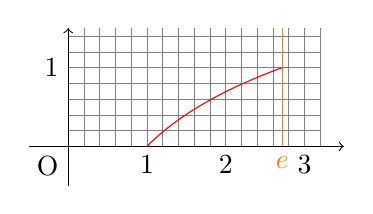
\begin{tikzpicture}
\draw[help lines,step=0.2] (0,0) grid (3.2,1.5);
\node[anchor=north east] at (0,0) {O};
\foreach \x in {1,2,3}
 \node[anchor=north] at (\x,0) {\x};
\foreach \y in {1}
 \node[anchor=east] at (0,\y) {\y};
 
\draw[->] (-0.5,0) -- (3.5,0);
\draw[->] (0,-0.5) -- (0,1.5);
\draw[-,color=orange] (2.71828,0) -- (2.71828,1.5);
\node[anchor=north,color=orange] at (2.71828,0) {$e$};
\draw[scale=1,domain=1:2.71828,smooth,variable=\x,red]  plot (\x,{ln(\x)});
\end{tikzpicture}
\end{center}

\exercise{37} ***
\[\int_{y=0}^4 \int \int\]

\subsection{Definition of Riemann Integral in $\R^n$}

\begin{defn}{Support of a function}
	The \ul{support} $\Supp(f)$ of a function $f : \R^n \to \R$ is the closure of the set
	\begin{equation}
		\Set{x\in\R^n \mid f(x)\neq 0}
	\end{equation}
\end{defn}

***

\begin{itemize}
	\item Partition $\R^n$ into cubes of side length 1. 	\[ \text{"cube"} = \mtrx{a_1, b_1} \times \mtrx{a_2, b_2} \times \cdots \times \mtrx{a_n, b_n}\]
	
	\item Refinement of this partition is obtained by subdividing each cube into $2^n$ subcubes of side length $\frac{1}{2}$, using the midpoints of each side. 
	\item We can then continue refining this partition to get cubes of arbitrarily small side length (and thus volume). 
\end{itemize}

Recall that
\begin{equation}
	\text{vol}_n \System{\mtrx{a_1, b_1} \times \cdots \times \mtrx{a_1, b_1}}=\prod_{i=1}^n |b_i-a_i|
\end{equation}

\begin{defn}{$N$th upper sum, $N$th lower sum} 
	Let $f: \R^n \to \R$ be bounded with bounded support. The $N$th \ul{upper} and \ul{lower sums} of a function $f$ are ***
	\begin{equation}
		U_N(f) 
	\end{equation}
\end{defn}

\begin{proposition}
	As $N$ increases, the sequence $N\mapsto U_N(f)$ is nonincreasing, and the sequence $N\mapsto L_N(f)$ is nondecreasing. 
\end{proposition}

\begin{defn}{Upper and lower integrals}
	We call
	\begin{equation}
		U(f)\overset{def}{=} \lim_{N\to \infty} U_N(f) \quad \text{and}\quad L(f)\overset{def}{=} \lim_{N\to \infty} L_N(f)
	\end{equation}
	the \ul{upper} and \ul{lower integrals} of $f$. 
\end{defn}

\begin{proposition}
	If $f$, $g$ are bounded functions with bounded support and $f\leq g$, then
	\begin{equation}
		U(f)\leq U(g) \quad \text{and} \quad L(f)\leq L(g)
	\end{equation}
\end{proposition}

\begin{defn}{Integral}
	A function $f : \R^n \to \R$, bounded with bounded support, is \ul{integrable} if its upper and lower integrals are equal: its integral is then
	\begin{equation}
		\int_{\R^n} f|d^n\bm{x}| \overset{def}{=} U(f) = L(f)
	\end{equation}
\end{defn}

\begin{defn}{Integrable}
	$f$ is \ul{R-integrable} if there exists an $N_0$ such that $U_N(f) - L_N(f) < \epsilon$ for all $N\geq N_0$. 
\end{defn}

\begin{proposition}\textbf{(Rules for computing multiple integrals).} ***

\begin{enumerate}
	\item $f+g$
	\item scalar multiplication
	\item if $f\leq g$ then $\int f \leq \int g$
	\item $\left|\int f\right|\leq \int |f|$
\end{enumerate}
\end{proposition}

\begin{defn}{$n$-dimensional volume}
	When $\bm{1}_A$ is integrable, the \ul{$n$-dimensional volume} of A is
	\begin{equation}
		\text{vol}_n A \Def \int_{\R^n} \bm{1}_A |d^n \bm{x}|
	\end{equation}
\end{defn}

"indicator function" : $\bm{1}_A (x) = \begin{cases}
	1 &\text{if }x\in A \\
	0 &\text{if }x\not\in A
\end{cases}$

\begin{proposition} \bm{(Set with volume 0).} A bounded set $X\subset \R^n$ has volume $0$ if and only if for every $\epsilon > 0$ there exists $N$ such that ***
\begin{equation}
	\sum_{\substack{C\in D_N(\R^n) \\ C \cap X \neq \emptyset}} \Vol_n (C) \leq \epsilon
\end{equation}
\end{proposition}

\exercise{4.1.10} \begin{enumerate}[a.]
	\item What are the upper and lower sums $U_1(f)$ and $L_1(f)$ for the function
	\[f\Point{x \\ y} = \begin{cases}
		x^2 + y^2 & \text{if }0<x, y<1 \\
		0 & \text{otherwise}	\end{cases} \]
		
		Infimums, supremums ***: 
\begin{center}
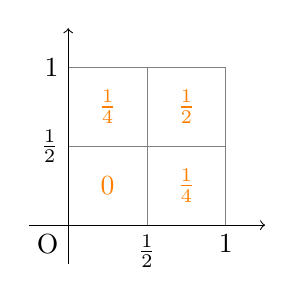
\begin{tikzpicture}
\draw[help lines,step=1] (0,0) grid (2,2);
\node[anchor=north east] at (0,0) {O};
\node[anchor=north] at (1,0) {$\frac{1}{2}$};
\node[anchor=north] at (2,0) {$1$};
\node[anchor=east] at (0,1) {$\frac{1}{2}$};
\node[anchor=east] at (0,2) {$1$};
 
\draw[->] (-0.5,0) -- (2.5,0);
\draw[->] (0,-0.5) -- (0,2.5);
\node[color=orange] at (0.5,0.5) {$0$};
\node[color=orange] at (1.5,0.5) {$\frac{1}{4}$};
\node[color=orange] at (0.5,1.5) {$\frac{1}{4}$};
\node[color=orange] at (1.5,1.5) {$\frac{1}{2}$};
\end{tikzpicture}
\[L_1(f) = \frac{1}{4}\left(0+\frac{1}{4}+\frac{1}{4}+\frac{1}{2}\right)=\frac{1}{4}\]

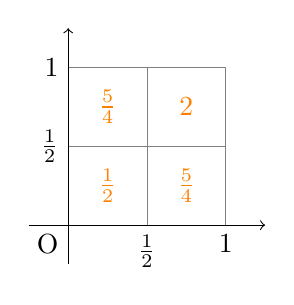
\begin{tikzpicture}
\draw[help lines,step=1] (0,0) grid (2,2);
\node[anchor=north east] at (0,0) {O};
\node[anchor=north] at (1,0) {$\frac{1}{2}$};
\node[anchor=north] at (2,0) {$1$};
\node[anchor=east] at (0,1) {$\frac{1}{2}$};
\node[anchor=east] at (0,2) {$1$};
 
\draw[->] (-0.5,0) -- (2.5,0);
\draw[->] (0,-0.5) -- (0,2.5);
\node[color=orange] at (0.5,0.5) {$\frac{1}{2}$};
\node[color=orange] at (1.5,0.5) {$\frac{5}{4}$};
\node[color=orange] at (0.5,1.5) {$\frac{5}{4}$};
\node[color=orange] at (1.5,1.5) {$2$};
\end{tikzpicture}
\[U_1(f) = \frac{1}{4}\left(\frac{1}{2}+\frac{5}{4}+\frac{5}{4}+2\right)=\frac{5}{4}\]
\end{center}
\end{enumerate}

Using Fubini's Theorem: 
\[\int_0^1 \int_0^1 x^2+y^2\ dy\ dx = \int_0^1 \left[ x^2y + \frac{1}{3}y^2 \right]_0^1 dx = \int_0^1 \left(x^2 + \frac{1}{3}\right)dx = \left[ \frac{1}{3}x^3 + \frac{1}{3}x \right]_0^1=\frac{2}{3}\]